\documentclass{standalone}
\begin{document}
	\subsection*{Training}
	
	This step involves the estimation of the centroid set. To achieve this purpose, a k-means clustering was performed on a training set made on multichannel images from many CT scans. During this task I have to takes into account that k-means clustering requires a balance in the different cluster representation. As we can see in \figurename\,\ref{fig:ClusterRepr}, the main part of the image is composed to background, that is an over-represented cluster. Moreover we can observe that the amount of involved lung volume may change according to the  severity of the disease: the first scan presents a low amount pf GGO and CS; the second one have a larger lung region involved.ù
	 
	\begin{figure}[h!]
		\centering
		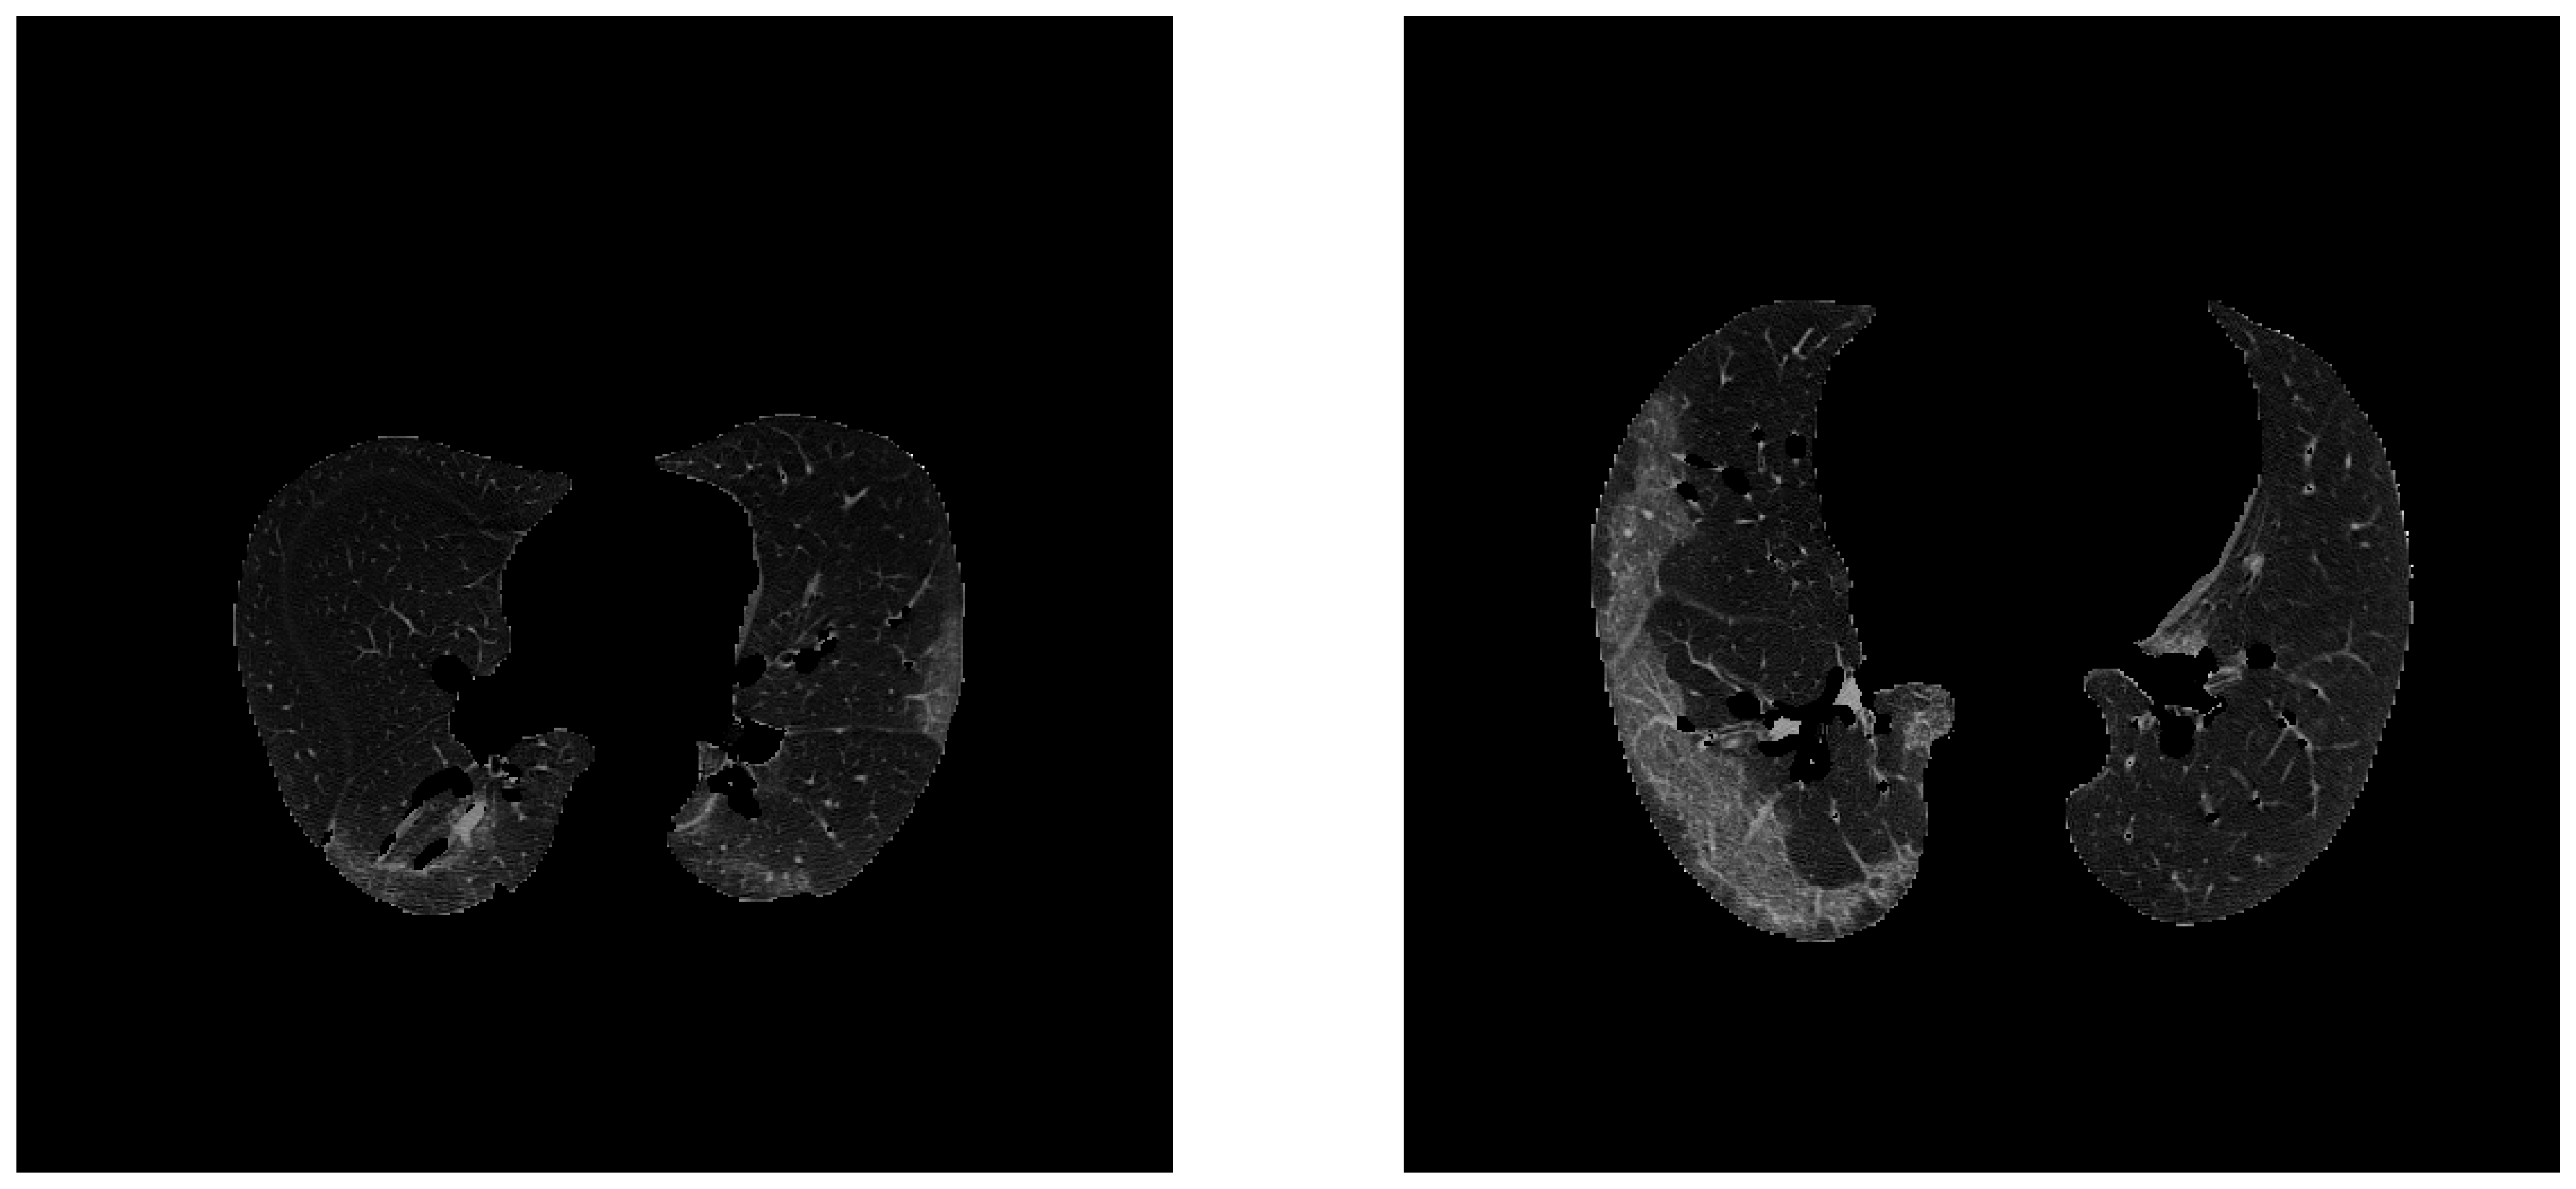
\includegraphics[scale=.4]{ClusterRepr.png}
		\caption{Lung regions with different ground glass areas. We can notice that the main part of the image is composed only by the background. From left to right respectively a scan with small lesion areas and one with a large lesion. }\label{fig:ClusterRepr}
	\end{figure}

	
	To overcome these issues, I have simply removed the background from the segmentation and carefully selected the scans of the training set to ensure a balanced representation of each cluster. The main rule used for the selection is that in each scan must be present a large lesion areas and also a well representation of artifacts, in order to takes into account all the possible features.
	
	The images of the training set are then shuffled and splitted into many subsamples and the clustering is performed independently on each one of them. As a final centroid set I have consider the one that minimize the intra cluster variance. This step is justified since the results of the k-means clustering depends on the initial choice centroids. During the minimization of the potential function the algorithm may find a local minimum rather than the global one. The different clustering allows to estimate more than one possible solution and to chose the best one. 		
	Moreover the creation of several sub-samples is made since the creation of a single, large array with several images is not always possible, since requires a huge quantity of memory to be allocated.
\end{document}	
